\chapter{Desenvolvimento}
    \label{chap:desenvolvimento}
    
    % implementação do porte
        % apresentação  da plataforma de hardware
        % EPOS, mediadores e abstrações
        % programação
        % depuração
    % implementação RT-DVS
    
    Este capítulo apresenta o desenvolvimento deste trabalho em duas seções. A primeira diz respeito ao porte do sistema operacional, apresentando o estudo de caso EPOS e suas características necessárias ao entendimento do capítulo, além da descrição da plataforma de hardware alvo escolhida. A segunda seção trata da criação de suporte a RT-DVFS sobre o sistema operacional EPOS já portado para a plataforma alvo.
    
    \begin{comment}
    \section{Porte do Sistema Operacional}
        \subsection{EPOS e Portabilidade}
            % Overview do que é o EPOS
            % Conceito de mediadores
            % Conceito de abstrações
        
        \subsection{Plataforma Alvo}
            \subsubsection{Programação}
            \subsubsection{Depuração}
            \subsubsection{Suporte a DVFS}

        \subsection{Run-time C++}
        \subsection{Inicialização do EPOS}
        \subsection{Implementação de Mediadores}
        \subsection{Mediador de Máquina e DVFS}
        
    \section{Criação do Ambiente RT-DVFS}
    \end{comment}
            
    \section{Porte do Sistema Operacional}
        \label{sec:plataforma}
        
        Esta seção apresenta a avaliação de uso da plataforma Gumstix Connex \cite{gumstix-legacy}, que possui um processador Intel PXA255 \cite{pxa255-developers-manual}, com a arquitetura Intel XScale, vastamente utilizada em estudos de energia na última década \cite{Chen:2007}. Além disso, também é descrita a estruturação do sistema EPOS necessária para o desenvolvimento do porte para a plataforma de hardware citada.
        
        \subsection{EPOS e Portabilidade}
        
        O EPOS (\emph{Embedded Parallel Operating System}) \cite{Frohlich:2001} é um sistema operacional direcionado a aplicações embarcadas de alto desempenho. Segue a metodologia ADESD (\emph{Application-Driven Embedded System Design}), utilizando técnicas de orientação a aspectos e programação estática em busca de se adequar às restrições presentes nas aplicações para o qual é utilizado.
        
        Ao mesmo tempo que o EPOS busca a especialização para a aplicação, deve lidar com a gama de plataformas utilizadas para a produção e durante o ciclo de vida das aplicações. O sistema operacional hoje, conta com portes para diversas plataformas, como IA32, ARM7, AVR8, MIPS e PowerPC. Seguindo a metodologia ADESD, ou seja, sendo um sistema orientado a aplicação, a troca da plataforma a ser utilizada na aplicação deve permanecer transparente ao programador do sistema.
        
        O EPOS busca balanço entre desempenho e portabilidade através de dois artefatos: primeiro, rotinas de pré-configuração, presentes no sistema como a entidade \emph{Setup Utility}; em segundo, os mediadores de hardware.
        
        \subsubsection{\emph{Setup Utility}}
            \label{sec:setup-utility}
        
        As rotinas de pré-configuração do sistema são porções de código dependentes de hardware. Elas são executadas anteriormente ao ambiente do sistema operacional. Seu papel é construir o contexto fundamental para a execução do EPOS. Isto significa oferecer um cenário seguro de execução e inicialização do sistema, garantido, por exemplo, a existência de uma pilha consistente ou o desligamento de interrupções. Estas rotinas facilitam a portabilidade devido ao fato de reduzirem a complexidade de outros componentes do sistema operacional.
        
        Ao final da execução do componente \emph{Setup Utility}, o controle do sistema é entregue ao suporte dinâmico (\emph{run-time}) da linguagem C++ (linguagem na qual maior parte do sistema é escrita), que desencadeia a inicialização dos outros componentes do EPOS.
        
        \subsubsection{Mediadores de Hardware}
        
        Os mediadores de hardware do EPOS oferecem interfaces simples para acesso a itens dependentes de máquina. Assim, componentes mais abstratos do sistema (chamados de \emph{abstrações}), como por exemplo, \emph{Thread} ou \emph{Scheduler}, podem permanecer com suas implementações portáveis independentemente da plataforma alvo.
        
        % Apresentados estes artefatos, conclui-se que, para a criação de um novo porte do sistema EPOS, basta implementar as rotinas de pré-configuração e os mediadores de hardware necessários aos componentes de mais alto-nível utilizados.

        \subsection{Plataforma Alvo}
            \label{sec:plataforma-alvo}
        
            A plataforma Connex faz parte de uma linha descontinuada de placa-mães da companhia Gumstix. Esta placa possui um processador Intel PXA255 com microarquitetura Intel XScale. O PXA255 mostrou-se interessante para os fins deste trabalho, pois o núcleo Intel XScale é justamente direcionado para aplicações embarcadas que exijam alta performance e baixo consumo de energia \cite{pxa255-developers-manual}.
            
            % Acrescentar uma figura da arquitetura interna de barramento/CPU/memória.
            
            O processador PXA255 suporta DVFS para três componentes do processador: a CPU, o barramento principal e memória \cite{Snowdown:2005}, fator fundamental para o desenvolvimento deste trabalho. Além disso:
            
            \begin{itemize}
                \item O laboratório onde este trabalho foi desenvolvido possui um conjunto de placas Connex e outros módulos de expansão.
                \item Mesmo com o processador PXA255 oferecendo uma interface JTAG \cite{jtag-standard} para depuração, as placas da linha Connex não oferecem acesso necessário a este recurso. Por outro lado, estas placas Gummstix podem ser emuladas através do QEMU \cite{qemu-website}. Felizmente, o QEMU possui opções de depuração junto ao GDB \cite{gdb-website}, de modo que seja possível a supervisão da execução de instruções passo a passo na plataforma.
                \item Processadores compatíveis com o PXA255 e sua arquitetura já estão bem estabelecidos na comunidade de sistemas embarcados e RT-DVFS. Muitos trabalhos exibem experimentos utilizando a plataforma \cite{Chen:2007}. Mesmo que a linha Connex tenha sido descontinuada no ano de 2009 pela Gumstix, ainda assim, versões recentes de placa-mães do mesmo fabricante utilizam arquiteturas compatíveis com a Intel XScale \cite{gumstix-products}. Assim sendo, além de um cenário de estudo presente em outras publicações, o projeto EPOS também se beneficia, já que o sistema será portado para uma plataforma que é amplamente utilizada em aplicações embarcadas que necessitam de baixo consumo de energia e alto desempenho.
                \item A arquitetura Intel XScale utiliza o conjunto de instruções ARMv5TE, mantendo compatibilidade binária com o conjunto ARMv4T \cite{arm-arm}. Felizmente o EPOS já possui porte para plataformas ARM7, sendo que estas seguem a arquitetura ARMv4T. Assim, é possível herdar parte considerável do suporte de baixo nível necessário ao EPOS e também reaproveitar a implementação de alguns componentes, como o mediador de CPU, responsável, por exemplo, pelas rotinas de troca de contexto.
            \end{itemize}
            
            A Gumstix Connex foi escolhida como plataforma de implementação deste trabalho, não somente por oferecer o suporte a DVFS, mas também pelos fatores facilitadores de implementação, além de benefícios experimentais ao EPOS.
                
        \subsection{Programação da Plataforma}
            \label{sec:programacao}
        
        Os primeiros passos tomados para portar o sistema operacional EPOS foram na direção da programação da plataforma Connex. Ela possui 64MB de RAM e uma memória \emph{flash} programável de 128kB, onde o processador busca, em seu endereço base, a primeira instrução para inicialização do sistema.
      
        De qualquer modo, esta memória programável já vem, desde a fabricação da plataforma, tomada pelo U-Boot, um \emph{bootloader} que facilita a inicialização de sistemas operacionais na plataforma. É necessário citar que o U-Boot possui rotinas que auxiliam na programação do sistema, como escrita em memória RAM ou própria \emph{flash}, sendo possível até carregar imagens executáveis utilizando o protocolo Kermit, isto através da porta serial disponível em uma das placas de expansão da plataforma Connex.
        
        Como a placa Connex não oferece acesso à interface JTAG oferecida pelo PXA255, a qual facilitaria a escrita da \emph{flash}, a melhor alternativa para programação da plataforma foi a utilização do próprio U-Boot. A partir da imagem de memória resultante da compilação do EPOS, que contém o sistema operacional, pode-se criar uma outra compatível com a rotina inicializadora de imagens do \emph{bootloader}. Para tanto, usa-se a ferramenta \emph{mkimage}. Criando a imagem EPOS compatível com o U-Boot, basta carregá-la em memória, utilizando a porta serial através do protocolo Kermit implemetado pelo U-Boot.
        
        \subsection{Depuração}
        
        Confirmado o método de programação da plataforma, procurou-se então testar as facilidades de depuração oferecidas pelo QEMU versão \emph{0.12.5}.
        
        O QEMU necessita de que uma imagem da memória programável seja especificada, logicamente para que a plataforma emulada seja inicializada conforme os moldes da seção anterior (\ref{sec:programacao}). Para que a emulação seja a mais fiel possível à plataforma disponível no laboratório, esta imagem foi criada com a versão \emph{1.2.0} do U-Boot, a mesma presente na placa Connex utilizada para desenvolvimento.
        
        A facilidade ofertada pelo QEMU é colocar-se como monitor remoto do GDB. Assim, é possível conectar o GDB (utilizando TCP) ao QEMU, e supervisionar a execução passo a passo de instruções na plataforma emulada. Até a programação pode ser feita através do GDB, escrevendo a imagem EPOS inicializável na memória emulada, e então, delegando ao U-Boot a inicialização do EPOS.
        
        Com os processos de programação da plataforma e depuração, o suporte técnico necessário para construção do novo porte é concluída.
        
        \subsection{\emph{Setup Utility} e \emph{Run-time C++}}
            \label{sec:setup-e-run-time}

         Para os fins deste projeto, o EPOS é configurado para uso em modo \emph{library}. Isto significa que ele é ligado à aplicação como uma biblioteca estática. Sendo assim, por exemplo, não há a necessidade do uso de chamadas de sistema (usualmente nomeadas \emph{System Calls}) \cite{Frohlich:2001}. 
         
         Para a inicialização do sistema operacional, basta indicar ao U-Boot o endereço da primeira instrução contida na imagem do EPOS. Em seu fluxo normal de inicialização, fluxo \emph{a} na figura \ref{fig:inicializacao-do-EPOS}, \emph{Setup Utility} é o primeiro componente do sistema a entrar em ação. No presente trabalho, pelos motivos apontados a seguir, elimina-se o componente \emph{Setup Utility}, seguindo o fluxo \emph{b} apresentado na figura \ref{fig:inicializacao-do-EPOS}.

        \begin{figure}[h]
        \centering
        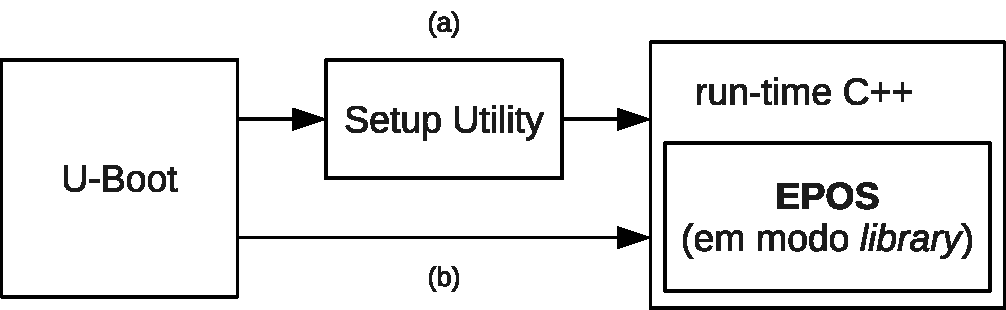
\includegraphics[scale=0.6]{imagens/inicializacao-do-EPOS.pdf}
        \captionof{figure}{Sequência de inicialização do EPOS}
        \label{fig:inicializacao-do-EPOS}
        \end{figure}
        
         Observe que a mesma abordagem é utilizada em outros portes, como por exemplo os para máquinas com arquitetura AVR8, que possuem também uma baixa complexidade relativa.
         
         \subsubsection{Remoção do \emph{Setup Utility}}
         
         Como explicado anteriormente em \ref{sec:setup-utility}, o EPOS possui uma rotina de pré-configuração do hardware. O objetivo dessa rotina é reduzir a complexidade de alguns componentes mais abstratos do sistema operacional. Se comparada a outras plataformas para quais o EPOS foi portado, como IA32 ou PowerPC, o processador PXA255 possui uma complexidade relativamente reduzida, justificando a não necessidade da criação do componente \emph{Setup Utility} para este porte. 
         
         As atividades de pré-configurações reconhecidas como necessárias, para a execução segura do EPOS, foram: o estabelecimento de uma pilha única consistente e o remapeamento dos vetores de interrupção do processador. Para reduzir o tempo de desenvolvimento, estas duas atividades foram delegadas, respectivamente, ao suporte dinâmico da linguagem C++ e às rotinas de inicialização dos mediadores de hardware. O funcionamento destes mecanismos são explicados em subseções seguintes.
         
         \subsubsection{\emph{Run-time} C++}
            \label{sec:run-time-c++}
         
        O \emph{run-time} C++ necessário é responsável por um fator essencial do sistema: inicialização de componentes do sistema, como mediadores ou entidades mais abstratas.
         
        Algumas instâncias de componentes do sistema são tratados pela linguagem como objetos de escopo global, isto faz com que as suas inicializações sejam dependentes da implementação dos mecanismos dinâmicos da linguagem C++ \cite{Stroustrup:1997}. Em outras palavras, isto significa que deve haver a implementação em software do suporte para que estes componentes tenham suas rotinas de inicialização, que foram geradas pelo compilador C++, chamadas antes da execução da função inicial da aplicação.
        
        Este suporte de baixo-nível deve ser escrito em linguagem \emph{assembly}, e portanto é dependente de arquitetura. Felizmente, como foram realizados trabalhos anteriores com processadores de arquitetura ARMv4T, aproveitou-se a compatibilidade binária, pois ARMv4T é um subconjunto das instruções ARMv5TE \cite{arm-arm}, utilizadas na arquitetura Intel XScale.
        
        Aproveitou-se o \emph{run-time} C++ para se adicionar as rotinas responsáveis pela manutenção da pilha do sistema. A arquitetura ARM possui um comportamento indefinido para acessos desalinhados à memória principal. Garantiu-se então, na inicialização da pilha, um endereço alinhado para a mesma. O código gerado pelo compilador faz a manutenção desta propriedade.
        
        Além disso, na arquitetura ARMv5TE, o processador possui pilhas diferenciadas para diversos modos de funcionamento. Isto significa que a pilha utilizada no tratamento de interrupções é diferente da pilha utilizada pela aplicação. Como o EPOS é utilizado em modo \emph{library} neste trabalho, a aplicação e o tratador de interrupções dividem o mesmo espaço de memória, ou seja, devem ser executados em um único modo de operação do processador, com uma única pilha. Como isso não é possível pelo funcionamento padrão da arquitetura, uma adaptação técnica foi realizada no \emph{run-time} C++ para que a existência de uma única pilha fosse transparente ao sistema EPOS.
        
        \subsection{Implementação de Mediadores}
            \label{sec:implementacao-de-mediadores}
        
        Os mediadores do EPOS são a interface para a acesso de componentes da plataforma de hardware \cite{Frohlich:2001}. Assim como as rotinas de pré-configuração, cada mediador é um componente do sistema dependente de máquina. De fato, a implementação dos mediadores para a plataforma PXA255 é o passo final e fundamental para a criação do porte.
        
        Para os fins deste trabalho, não necessariamente todos os mediadores do sistema precisam ser implementados. Isso acontece porque as abstrações que serão utilizadas para experimento estão restringidas a componentes de processo e tempo. Não é preciso, por exemplo, que se implemente mediadores para a interface \emph{bluetooth}, pois sincronizadores, escalonadores, etc. não utilizam este tipo de mediador.
        
        \begin{figure}[h]
        \centering
        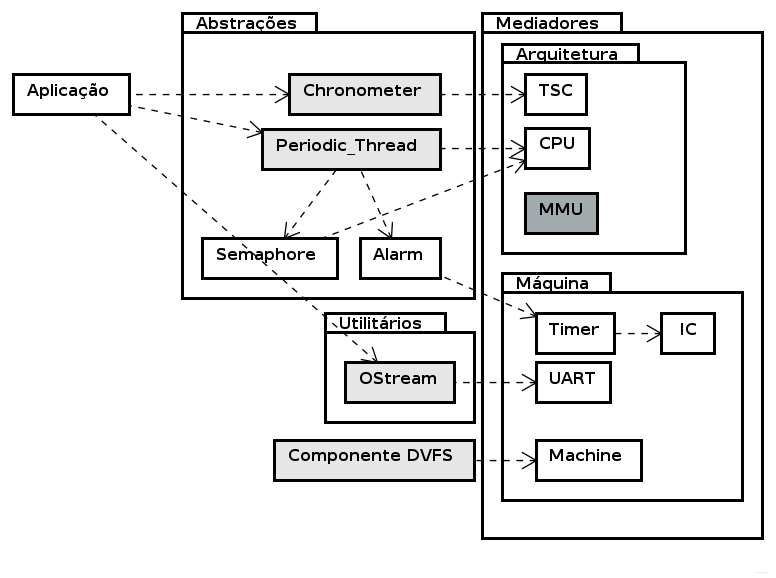
\includegraphics[scale=0.6]{imagens/dependencias-de-mediadores.png}
        \captionof{figure}{Análise de dependências entre aplicação, abstrações e mediadores para o porte}
        \label{fig:dependencias}
        \end{figure}
        
        Em uma análise para definir os mediadores necessários, o diagrama de classes apresentado na figura \ref{fig:dependencias} foi desenvolvido. A aplicação criada posteriormente para experimentos utiliza diretamente somente duas abstrações: \emph{Periodic\_Thread} (tarefas periódicas) e \emph{Chronometer} (cronômetro virtual), além do utilitário \emph{OStream} (saída de dados). Estas dependências exigem, indiretamente, a implementação dos mediadores: \emph{CPU}, \emph{Timer} (temporizador), \emph{UART}, \emph{TSC} (contador temporizado) e \emph{IC} (controlador de interrupções).
        
        O mediador de \emph{MMU} foi também escolhido para implementação, pois foi delegado a ele o remapeamento dos vetores de interrupção (subseção \ref{sec:setup-e-run-time}), procedimento esclarecido mais adiante.
        
        O mediador \emph{Machine}, ou mediador de máquina, é responsável pelas características presentes no PXA255, mas que excedem o conceito de arquitetura (interface binária) do processador. Logo, as atividades de alteração de tensão e frequência devem ser atribuídas a este mediador.
        
        A seguir, são apresentadas informações breves sobre a implementação de cada um destes mediadores.
        
        \subsubsection{\emph{CPU}}
        
        Este mediador é responsável por características como a troca de contexto, entrada e saída em registradores, habilitação de interrupções, e criação de pilhas para novas \emph{threads} no sistema. Sendo assim, é um mediador intimamente ligado com as questões de gerenciamento de tarefas no EPOS. Boa parte deste mediador pôde ser herdada do suporte às arquiteturas ARM utilizadas em projetos anteriores. Ainda assim, pequenas modificações foram necessárias, pois algumas operações de entrada e saída envolvem coprocessadores específicos da arquitetura Intel XScale.
        
        \subsubsection{\emph{Timer}}
        
        Este mediador é requerido por várias abstrações relacionadas a processos, como por exemplo, escalonadores ativos. Como a abstração \emph{Periodic\_Thread} necessita de invocações periódicas, este mediador necessita de implementação.
        
        \subsubsection{\emph{UART}}
        
        O EPOS utiliza este mediador muito cedo em sua inicialização, de modo que seja possível facilitar a depuração em máquinas reais, onde o uso de emuladores e JTAG pode não ser uma realidade. Utilizando a placa Connex em conjunto com sua expansão HWUART, é possível obter informações do sistema em tempo de execução.
        
        \subsubsection{\emph{TSC}}
        
        O TSC (\emph{Time Stamp Counter}) é um dispositivo que auxilia a medição de tempo em alta resolução.
        
        \subsubsection{\emph{IC}}
        
        A arquitetura ARM necessita de um roteamento de interrupções em alto nível. Este mediador abstrai itens referentes aos indicadores de interrupção da máquina, para a decisão de qual tratador instalado chamar. Este mediador é necessário para o funcionamento ideal, por exemplo, do mediador \emph{Timer}.
        
        \subsubsection{\emph{MMU}}
        
         Por padrão, os processadores ARM (como é o caso do Intel XScale) utilizam um vetor de interrupções que encontra-se no endereço 0 emitido pela CPU. Como na máquina Connex este endereço refere-se à \emph{flash} programável, onde já encontra-se instalado um vetor de interrupções do U-Boot, é preciso que seja configurado, através da MMU presente no PXA255, um remapeamento dos endereços emitidos (virtuais) para novos endereços físicos. Assim, é possível traduzir o endereço padrão do vetor de interrupções (endereço 0), que está em \emph{flash}, para um endereço qualquer em RAM, sendo possível instalar nesta memória um vetor de interrupções apropriado ao EPOS.
         
         A MMU do PXA255 segue a VMSAv5 (\emph{Virtual Memory System Architecture version 5}), como descrita no \emph{Arm Reference Manual} \cite{arm-arm}. Na inicialização do mediador de MMU, foi inserida uma rotina que preenche a tabela de descritores de memória. Esses descritores fazem o remapeamento da faixa inicial de 1MB de memória em \emph{flash}, para a primeira faixa de 1MB em RAM. Assim, sempre que uma interrupção for chamada, o acesso ao endereço virtual 0, onde se encontra o vetor de interrupções do U-Boot, será na realidade um acesso ao endereço real em RAM, onde o vetor de interrupções preenchido pelo EPOS se encontra.

        \subsubsection{\emph{Machine}}
        
        Este mediador refere-se ao PXA255 e seus componentes. É ele que deve possuir a interface para que o modo de operação do processador seja alterado. A seção \ref{sec:suporte-dvfs} explica com mais detalhes a implementação do suporte a DVFS.
        
        \subsection{Implementação do Suporte a DVFS}
            \label{sec:suporte-dvfs}
        
        Como citado na seção \ref{sec:plataforma-alvo}, o PXA255 possui suporte a alteração dinâmica de frequência e tensão para três dispositivos: núcleo do processador, barramento do sistema (\emph{PXBus}) e memória SDRAM. A relação entre os principais componentes do PXA255 pode ser observada na figura \ref{fig:arquitetura-do-pxa}. Na mesma figura, em destaque, encontram-se os dispositivos que suportam DVFS.
        
        \begin{figure}[h]
        \centering
        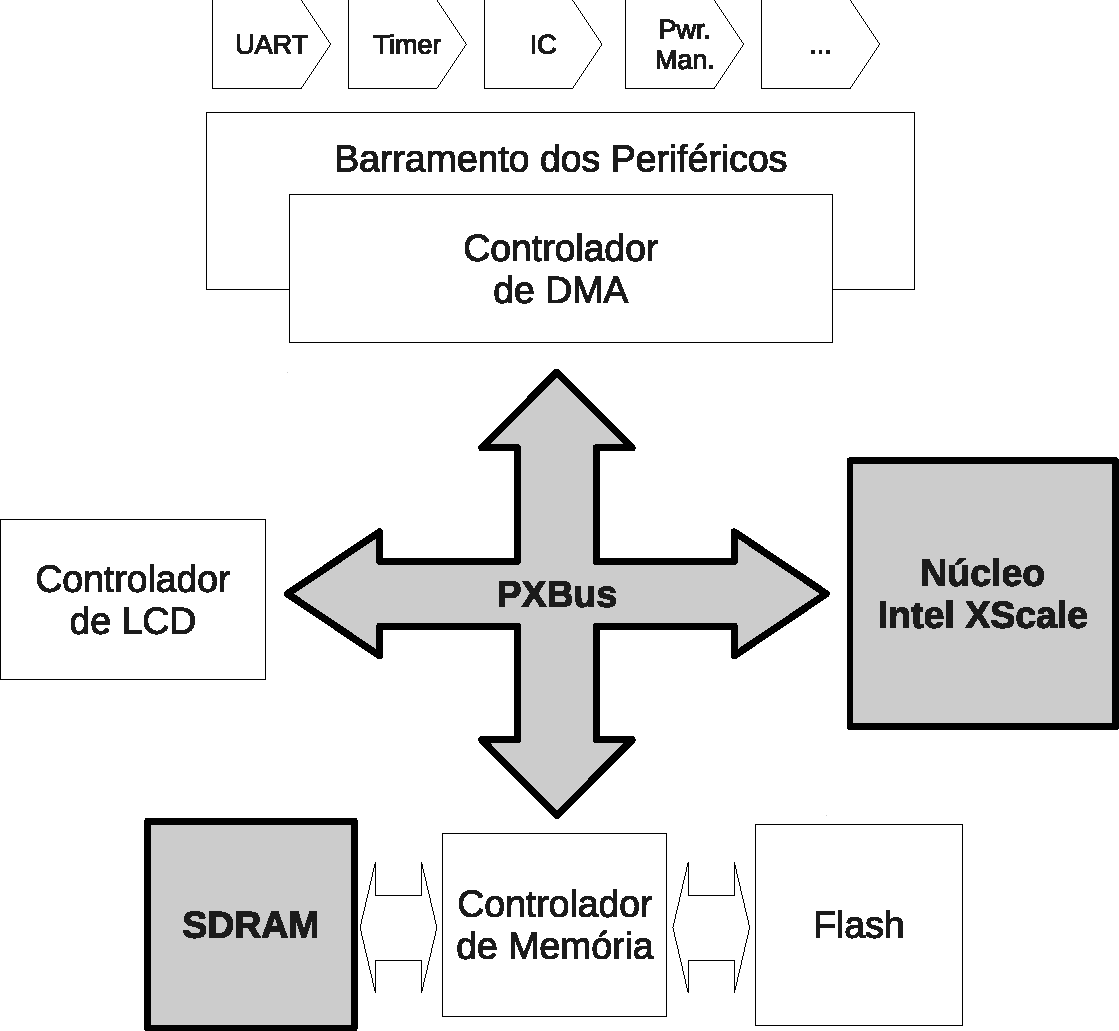
\includegraphics[scale=0.5]{imagens/arquitetura-do-pxa.pdf}
        \captionof{figure}{Representação dos componentes do processador PXA255}
        \label{fig:arquitetura-do-pxa}
        \end{figure}
        
        Segundo o \emph{Intel PXA255 Developer's Manual} \cite{pxa255-developers-manual}, existe um conjunto de configurações de frequência válidas para estes dispositivos. Este conjunto é apresentado na tabela \ref{tab:configuracoes}.
        
        %\begin{center}
        \begin{table}
        \begin{tabularx}{\textwidth}{ |C|C|C|C| }
            \hline
            Tensão do processador ($V$)&
            Frequência do Núcleo ($MHz$)&
            Frequência do PXBus ($MHz$)&
            Frequência da SDRAM ($MHz$)\\ \hline \hline
            1.0 & 99,5 & 50 & 99,5 \\ \hline
            1.0 & 199,1 & 50 & 99,5 \\ \hline
            1.1 & 298,6 & 50 & 99,5 \\ \hline
            1.0 & 132,7 & 66 & 66 \\ \hline
            1.0 & 199,1 & 99,5 & 99,5 \\ \hline
            1.1 & 298,6 & 99,5 & 99,5 \\ \hline
            1.3 & 398,1 & 99,5 & 99,5 \\ \hline
            1.1 & 265,4 & 132,7 & 66 \\ \hline
            1.3 & 331,8 & 165,9 & 83 \\ \hline
            1.3 & 398,1 & 186 & 99,5 \\ \hline
        \end{tabularx}
        \captionof{table}{Possíveis configurações de tensão e frequência para o PXA255}
        \label{tab:configuracoes}
        \end{table}
        %\end{center}
        
        No PXA255, a alteração dinâmica de frequência e tensão é feita através da FCS (\emph{Frequency Change Sequence}). Para qualquer alteração na configuração corrente do processador, invocando a FCS, os seguintes passos devem ser executados diretamente por software \cite{pxa255-developers-manual}:
        
        \begin{enumerate}
            \item Configurar o controlador de memória para que a frequência de atualização da SDRAM seja compatível com as frequências anterior e posterior à FCS.
            \item Desabilitar o controlador de LCD.
            \item Configurar os periféricos para que eles manipulem o atraso que a FCS pode ocasionar no controlador de DMA.
            \item Desabilitar periféricos que não podem acomodar um atraso maior que 500$\mu s$ no tratamento de suas interrupções. Isto se dá porque todas interrupções geradas durante a FCS são tratadas apenas ao final do processo de configuração.
            \item Programar o registrador CCCR (\emph{Core Clock Configuration Register}), de modo a representar uma das configurações apresentadas na tabela \ref{tab:configuracoes}.
            \item Invocar a FCS através da escrita do primeiro bit à direita do registrador CCLKCFG.
        \end{enumerate}
        
        Após a execução do item 6, o fluxo de execução de instruções continua normalmente. Os itens 2, 3 e 4 foram ignorados para a implementação deste porte, pois os controladores de LCD e DMA não foram utilizados em nenhum momento. Além disso, o tratamento de interrupções não foi prejudicado conforme o especificado no item 4.
        
        Para algumas das configurações apresentadas na tabela \ref{tab:configuracoes}, não basta apenas a invocação da FCS pelo registrador CCLKCFG, mas também a invocação do modo \emph{TURBO}, realizada pela escrita do segundo bit à direita do mesmo registrador.
        
        Os métodos para invocação da FCS e do modo TURBO foram encapsulados no mediador de máquina, conforme apresentado no diagrama de classes da figura \ref{fig:mediador-pxa255}.
        
        \begin{figure}[h]
        \centering
        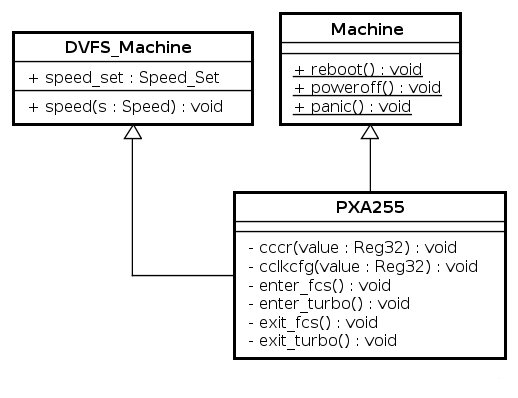
\includegraphics[scale=0.6]{imagens/mediador-pxa255.png}
        \captionof{figure}{Diagrama de classes do mediador de máquina para PXA255}
        \label{fig:mediador-pxa255}
        \end{figure}
        
        Para facilitar a interação entre heurísticas DVFS e o mediador de máquina, uma interface chamada \emph{DVFS\_Machine} foi criada. Essa interface é capaz de fornecer às abstrações do sistema as configurações disponíveis e um meio de aplicá-las. É ela a responsável pelo cumprimento dos passos descritos na enumeração anterior.
           
    \section{Criação do Ambiente RT-DVFS}
        
        Para a adequação com o modelo de sistema de tempo real apresentado na seção \ref{sec:modelo-de-sistema-de-tempo-real}, é utilizada a abstração do EPOS chamada \emph{Periodic\_Thread}. Uma extensão para seu funcionamento foi criada, de modo a captar-se os eventos necessários para a implementação das heurísticas \emph{Cycle-conserving DVS} para EDF e \emph{Static Voltage Scaling} para EDF.

        \subsection{\emph{Threads} Periódicas no EPOS}
            \label{sec:threads-periodicas-no-epos}
        
        A abstração \emph{Periodic\_Thread} do EPOS oferece suporte à execução periódica de tarefas no sistema. A partir dessa abstração, é possível criar um objeto ao qual existem associados um período e uma rotina a ser executada. Este período é representado, na imagem \ref{fig:periodic-thread}, como sendo o atributo \emph{period} da classe \emph{Alarm}. A rotina associada à tarefa periódica é representada na mesma imagem pelo atributo \emph{entry}, herdado por \emph{Periodic\_Thread} da classe \emph{Thread}.
        
        \begin{center}
        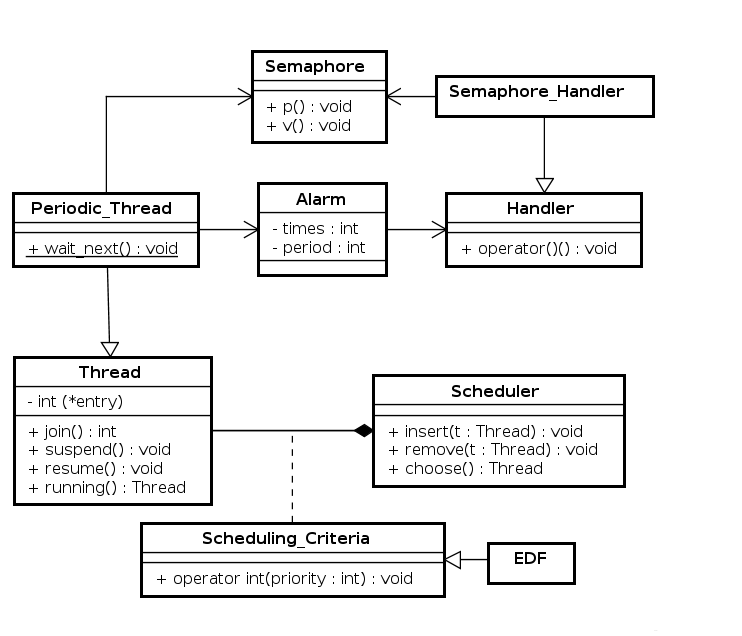
\includegraphics[scale=0.6]{imagens/periodic-thread.png}
        \captionof{figure}{Diagrama de classes apresentando a abstração \emph{Periodic\_Thread}}
        \label{fig:periodic-thread}
        \end{center}
        
        A rotina a ser executada periodicamente deve ser uma função C++ não-membro \cite{Stroustrup:1997}, que deve explicitamente se comportar como um laço, invocando dentro do bloco de repetição a função membro estática \emph{Periodic\_Thread::wait\-\_next}. O exemplo a seguir (\ref{tarefa}) demonstra este artefato para um número \textit{iterations} de repetições da tarefa. Observe que é possível estratificar a execução da tarefa em um ponto para sua inicialização, outro ponto com o corpo de código que será executado repetidamente, e por final, um trecho de código que representa a finalização da tarefa.
        
        
        \begin{lstlisting}[label=tarefa, escapeinside='', float=b, captionpos=b, caption=Exemplo de uma tarefa como uma função não-membro]
        int periodic_task(int iterations){
        
            // inicializa'\textit{çã}'o
            
            for(int i = 0; i < iterations; i++){
                // corpo da tarefa
                Periodic_Thread::wait_next();
            }
            
            // finaliza'\textit{çã}'o
            
            return 0;
        }
        \end{lstlisting}
        
                               
        A \emph{thread} que executa a função membro \emph{Periodic\_Thread::wait\_next}, através da operação ``\emph{p}'' sobre semáforo associado à abstração \emph{Periodic\_Thread}, perde o processador. Esta \emph{thread} entrará em um estado onde ela não ocupará mais a CPU até que a operação ``\emph{v}'' seja realizada sobre o mesmo semáforo. Para oferecer o comportamento periódico às tarefas, a abstração \emph{Alarm} é então utilizada. 
        
        A abstração \emph{Alarm} invoca periodicamente um objeto função (instância da classe \emph{Handler} apresentada na figura \ref{fig:periodic-thread}), neste caso especializado para executar a operação ``\emph{v}'' sobre o semáforo que ``impede'' a repetição do corpo do laço. A \emph{thread} pode então, voltar a ganhar a CPU segundo os critérios do escalonador. Ao recuperar a execução, ela volta ao ponto onde invocou \emph{Periodic\_Thread::wait\_next}, obedecendo ao comportamento do laço escrito.
        
        % Adicionar um diagrama de sequência para este parágrafo.
        
        O escalonador EDF entra como critério de ordenação utilizado pela classe \emph{Scheduler}, também apresentada na figura \ref{fig:periodic-thread}. Para configurar o critério utilizado no escalonamento, o EPOS utiliza o padrão de projeto \emph{traits}, oferecendo a escolha da política como uma configuração estática do sistema \cite{Frohlich:2001}.
        
        \subsection{Modificações no Modelo de \emph{Threads}}
        
        Para implementação das heurísticas para RT-DVFS, algumas modificações foram necessárias no sistema EPOS. Primeiramente, as heurísticas precisam estar cientes de eventos referentes às tarefas, como inicialização, término ou até mesmo alterações no conjunto de tarefas. Ainda, o sistema deve reagir a eventos como a troca de contexto, já que o modelo utilizado é preemptivo. Para que fosse possível atribuir ações a estes eventos, algumas modificações foram necessárias no modelo de \emph{threads} periódicas do EPOS, como apresentado no diagrama de classes da figura \ref{fig:ea-periodic-thread}.
        
        \begin{figure}[h]
        \begin{center}
        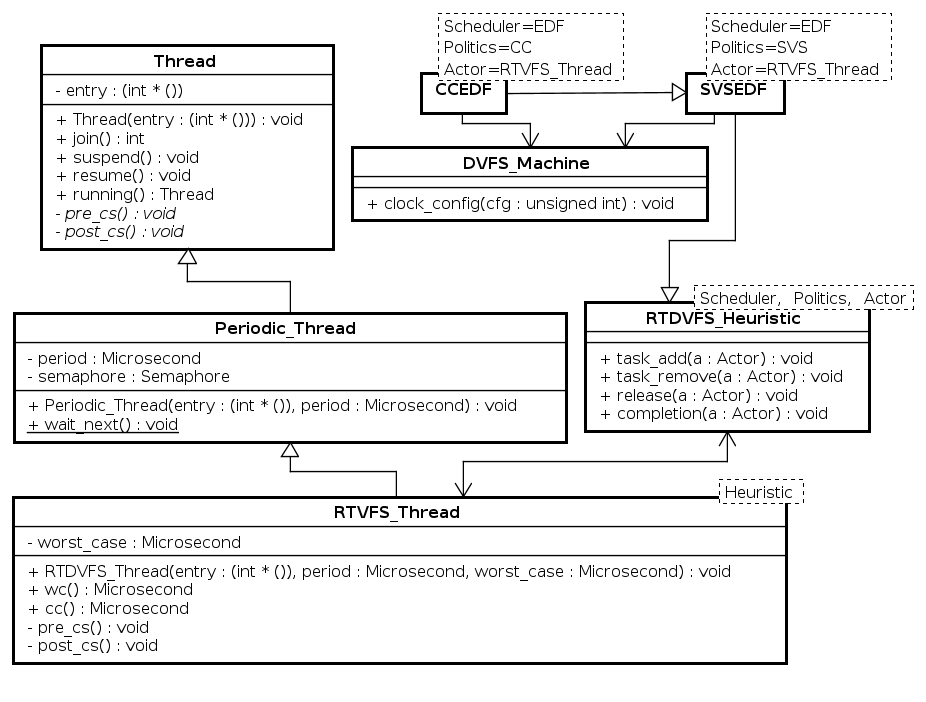
\includegraphics[scale=0.6]{imagens/ea-periodic-thread.png}
        \captionof{figure}{Diagrama de classes demonstrando as relações da \emph{EA\_Periodic\_Thread}}
        \label{fig:ea-periodic-thread}
        \end{center}
        \end{figure}
        
        Para reagir à troca de contexto, dois métodos foram criados na interface da classe \emph{Thread}: \emph{pre\_cs} e \emph{post\_cs}. Esses métodos são dedicados a extrair os pontos de execução antes e depois da troca de contexto entre \emph{threads}. Em C++, estes foram criados como funções membro virtuais, passíveis de serem sobrecarregados por classes filhas de \emph{Thread}. A interceptação destes eventos auxilia no cálculo do tempo de computação efetivamente utilizado pela tarefa.
        
        Para reagir aos outros eventos citados, a classe \emph{Periodic\_Thread} foi especializada. Uma filha chamada \emph{EA\_Periodic\_Thread} (do inglês \emph{Energy-aware Periodic Thread}) foi criada como uma abstração a fim de capturar estes eventos e repassá-los à heurística a ser utilizada. Ainda, a abstração \emph{EA\_Periodic\_Thread} recebe como parâmetros de construção o pior tempo de computação da tarefa que ela representa.
        
        \subsubsection{Captura de Modificações no Conjunto de Tarefas}
        
        A reação à alteração no conjunto de tarefas é dada a partir de duas maneiras: adição ou remoção de tarefas. Para capturar o evento de adição, em toda construção de uma nova \emph{EA\_Periodic\_Thread}, a classe \emph{Heuristic} tem o método \emph{task\_add} invocado, conforme apresentado no diagrama de sequência da figura \ref{fig:task-add}. Analogamente, na destruição de uma \emph{EA\_Periodic\_Thread}, o método \emph{task\_remove} é chamado.
        
        \begin{figure}
        \begin{center}
        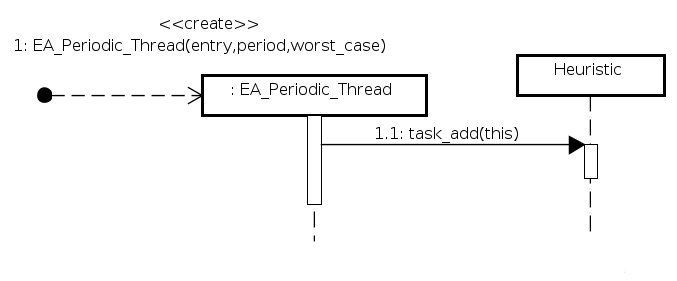
\includegraphics[scale=0.6]{imagens/task-add.png}
        \captionof{figure}{Diagrama de sequência demonstrando a criação de uma nova \emph{EA\_Periodic\-\_\-Thread}}
        \label{fig:task-add}
        \end{center}
        \end{figure}
        
        \subsubsection{Captura da Inicialização e Término de uma Tarefa}
        
        Os eventos de inicialização e término de tarefas são capturados através da reimplementação do método \emph{wait\_next} para a \emph{EA\_Periodic\_Thread}. O diagrama de sequência da figura \ref{fig:release-e-termination} mostra o momento em que estes eventos são reportados à heurística, anteriormente e posteriormente à aquisição de recurso no semáforo pertencente à \emph{thread} periódica (mecanismo explicado anteriormente na seção \ref{sec:threads-periodicas-no-epos}).
        
        \begin{figure}
        \begin{center}
        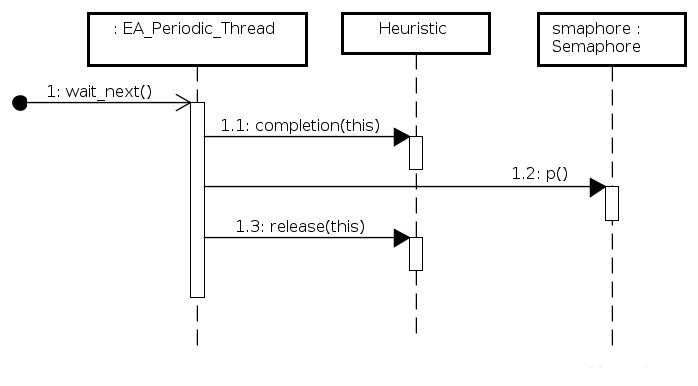
\includegraphics[scale=0.6]{imagens/release-e-termination.png}
        \captionof{figure}{Diagrama de sequência demonstrando o comportamento do método \emph{wait\_next} da classe \emph{EA\_Periodic\-\_\-Thread}}
        \label{fig:release-e-termination}
        \end{center}
        \end{figure}
        
        \subsubsection{Heurísticas}
        
        A implementação das heurísticas foram realizadas na forma de especialização de \textit{templates} em C++. A escolha da heurística pode ser programada estaticamente, sendo que cada heurística é uma especialização de três parâmetros: \emph{Scheduler} (o escalonador a ser usado, neste trabalho sempre EDF), \emph{Politics} (a política a ser utilizada: \emph{Static Voltage Scaling} ou \emph{Cycle-conserving}) e \emph{Actor} (a abstração que utiliza a heurística, neste trabalho sempre \emph{EA\_Periodic\_Thread}).
        
        \subsection{Implementação de \emph{Static Voltage Scaling} para EDF}
        
        Para implementar a heurística \emph{Static Voltage Scaling} para EDF, uma especialização \emph{SVSEDF} foi criada a partir da classe \emph{Heuristic} (figura \ref{fig:ea-periodic-thread}).
        
        A cada chamada de \emph{task\_add} ou \emph{task\_remove}, uma lista interna (\emph{periodics}) a \emph{SVSEDF} contendo objetos \emph{EA\_Periodic\_Thread} é atualizada. Quando este evento ocorre, o método \emph{select\_frequency}, escrito nos moldes do algoritmo \ref{alg:seleciona-frequencia}, é chamado. O trecho abaixo mostra o código em C++ do método citado:
        
        \begin{lstlisting}[label=select_frequency, escapeinside='', float=h, captionpos=b, caption=Método SVSEDF::select\_frequency]
        void SVSEDF::select_frequency(){
             
            EA_Periodic_Thread::List::iterator i; 
            double u = 0; // utiliza'\textit{çã}'o
            for(i = periodics.begin(); i != periodics.end(); i++){
                EA_Periodic_Thread* t = i->objetct();
                u += i->wc()/i->period();   // c'\textit{á}'lculo da utiliza'\textit{çã}'o
                                            // de pior caso
            }
            
            DVFS_Machine::Speed_Set::iterator j;
            for(j = DVFS_Machine::speed_set.begin();
                j != DVFS_Machine::speed_set.end();
                j++) {

                if(u <= j->objetct()->norm()){
                    DVFS_Machine::speed(*(j->objetct()));
                    return;
                }              
            }
            
            DVFS_Machine::speed(SVFS_Machine::max_speed());
        }
        \end{lstlisting}
        
        Observe que o método \emph{DVFS\_Machine::Speed::norm} é utilizado. Este método retorna a frequência normalizada de uma suposta configuração do tipo \emph{DVFS\_\-Machine::\-Speed}. Caso uma configuração de frequência normalizada menor ou igual a 1 não seja encontrada, a frequência máxima é utilizada.
        
        \subsection{Implementação de \emph{Cycle-conserving DVS} para EDF}
        
        Na implementação da heurística dinâmica, um método \emph{select\_frequency} também é implementado, mas neste caso, em vez do cálculo da utilização de pior caso, é feito o cálculo da utilização real quando a tarefa encontra-se terminada.

        \begin{lstlisting}[label=select_frequency, escapeinside='', float=h, captionpos=b, caption=Método CCEDF::select\_frequency]
        void CCEDF::select_frequency(){
             
            EA_Periodic_Thread::List::iterator i; 
            double u = 0; // utiliza'\textit{çã}'o
            for(i = periodics.begin(); i != periodics.end(); i++){
                EA_Periodic_Thread* t = i->objetct();
                if(!t->completed())
                    u += i->wc()/i->period();
                else
                    u += i->cc()/i->period();
            }
            
            //...
        }
        
        void CCEDF::completion(Actor* actor){
            select_frequency();
        }
        
        void CCEDF::release(Actor* actor){
            select_frequency();
        }
        \end{lstlisting}
        
        A heurística dinâmica também utiliza a adição e remoção de tarefas para atualizar a lista \emph{periodics}. Deste modo, a inicialização da execução do conjunto de tarefas sempre se dá com o processador configurado para o desempenho de pior caso de utilização. O efeito dinâmico é adquirido através da invocação de \emph{CCEDF::select\_frequency} pelos eventos de término e início de execução de das \emph{threads} periódicas.
            
            
